\documentclass[12pt,a4paper, flushleft]{article}
\usepackage[utf8]{inputenc}
\usepackage{amsmath,amssymb,amsthm}
\usepackage[T2A]{fontenc}
\usepackage[russian]{babel}
\usepackage{mathrsfs, dsfont} % специальные шрифты, по типу \mathscr или \dsfont
\usepackage{comment} %для многострочных комментариев
\usepackage{xcolor} %для гиперссылок в тексте и их цвета
\usepackage{hyperref}
\usepackage{graphicx}
\usepackage{wrapfig}
\usepackage{lipsum}
\usepackage{multicol}
\graphicspath{/home/cowberry/Documents/10M/SPTYM/pics/}
\usepackage[left=2cm,right=2cm,top=2cm,bottom=2cm]{geometry}	
\usepackage[most]{tcolorbox}
\definecolor{block-gray}{gray}{0.90} % уровень прозрачности (1 - максимум)
\newtcolorbox{myquote}{colback=block-gray,grow to right by=-25mm,grow to left by=-25mm, boxrule=1pt,boxsep=0pt,breakable}
\author{Анатолий Коченюк, команда ЛНМО\#2}
\date{Март 2019}
\title{Зодача \textsuperscript{\textregistered} №5}
\newcommand{\horline}[1]{
		\begin{center}
			\begin{picture}(#1, 2)
				\line(1,0){#1}%
			\end{picture}
		\end{center}
	}
\title{
	\vspace{4cm}	
	\horline{380}	
	\begin{center}
		\begin{Huge}
			\textbf{\emph{Задача 5. Крадущаяся змея, затаившееся полимино.}}
		\end{Huge}
	\end{center}	
	\vspace{-1.3cm}	
	\horline{400}
	%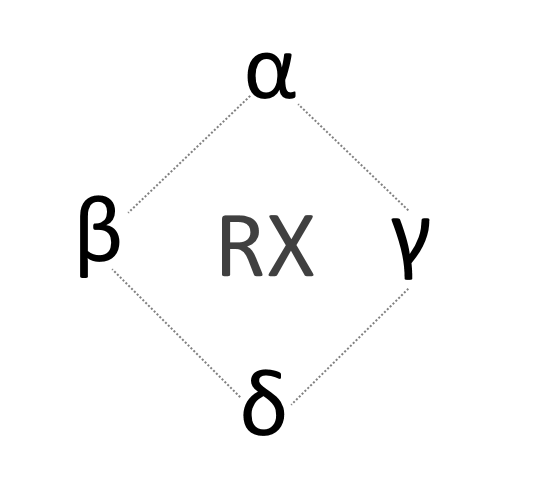
\includegraphics[scale=0.15]{abgrx.png}
}
\newtheorem{Def}{Определение}[section]
\newtheorem{Th}{Теорема}[section]
\newtheorem{Lm}{Лемма}[section] 
\newtheorem{Pb}{Задача}[section]
\newtheorem{Qu}{Признак}[section]
\newtheorem{St}{Утверждение}[section]
\newtheorem{Sl}{Следствие}[section]
\newtheorem{Zm}{Замечание}[section]
\newtheorem{Con}{Условие}[section]
\usepackage{relsize}
\newcommand{\vel}{\mathlarger{\mathlarger{\upsilon}}}
\newcommand{\der}[1]{\overset{\cdot}{#1}}
\newcommand{\dder}[1]{\overset{\cdot \cdot}{#1}}
\newcommand{\Lim}[2]{\lim\limits_{#1\to #2}}
\newcommand{\Ch}[1]{\overset{#1}{=}}
\newcommand{\p}[1]{#1^{\prime}}
\newcommand{\pp}[1]{#1^{\prime\prime}}
\newcommand{\ol}[1]{\overline{#1}}
\newcommand{\oll}[1]{\overline{\overline{#1}}}
\newcommand{\ov}[2]{\overset{#1}{#2}}
\newcommand{\un}[1]{\underline{#1}}
\newcommand{\gr}[2]{\includegraphics[scale=#1]{../pics/#2}}
\usepackage{comment}

\begin{document}
\maketitle
\vspace{4cm}
	
	\begin{myquote}
	\begin{center}
		\textbf{Аннотация}\\
		\textit{
			В этой статье полностью решён первый пункт, а также решена часть второго пункта.\\
			Были доказаны некоторые леммы, позволяющие удобно работать с эквивалентностью ломаных.
			Также были доказаны два условия того, что ломаная является кратчайшей.
		}
	\end{center}
	\end{myquote}	
	
	\pagebreak

	\tableofcontents	
	
	\pagebreak

\section*{Введение}

Рассмотрим множество ломаных на решётке $\mathds{Z}\times \mathds{Z}$ с началом в точке $(0, 0)$

\begin{enumerate}
	\item Ломаную можно представить как путь в $\{(x, y)\in\mathds{R}^2\mid x\in \mathds{Z} \text{ или } y\in\mathds{Z}\}$
	Введём специальные обозначения, для задания ломаной.
	\begin{enumerate}
		\item[] $a, A$ -- отрезки направленные вправо и влево
		\item[] $b, B$ -- вверх и вниз
	\end{enumerate}
	\item Общее количество таких отрезков будем называть длиной ломаной.
	\begin{enumerate}
		\item []Допускается случай ломанной с длиной 0 -- $\varepsilon$
	\end{enumerate}
	\item Ломаная замкнутая, если её конец совпадает с началом [$(0, 0)$]
	\item Ломаная простая, если у неё нет самопересечений по вершинам (допускается перечение начала и конца -- случай замкнутой ломаной)	
\end{enumerate}

Введём 2 операции над ломанными:
\begin{enumerate}
	\item Вытягивание и затягивание -- добавление в любое место пути $l\in\{aA, Aa, bB, Bb\}$
	\item Перенос -- мы можем свободно перемещать в любое место пути определённые комбинации. В Теории групп есть понятие описывающие такие конструкции -- коммутатор.
	
	Коммутатор -- для $f, g\in G$  $ [g, h] = ghg^{-1}h^{-1}$. 
	
	Если рассмотреть группу $G = \langle a, b\rangle$ (Положим, что $A = a^{-1}$ и $B = b^{-1}$)
\end{enumerate}

Говоря о теории групп, можно задать группу всех ломанных с учётом операций:

$G =\langle a, b\mid [x, y]z = z[x, y], x, y, z\in \{a, b, A, B\}\rangle\quad\quad $ (первая операция будет автоматически учтена, т.к. в группе произведение)

\begin{Def}
	Обратное слово -- конкатенация обратных элементов в обратном порядке
\end{Def}

\begin{Zm}
	Если два слова эквивалентны, то произведение первого на обратное ко второму эквивалентно пустому слову. 
\end{Zm}
\begin{proof}
	$l\equiv m$
	
	$lm^{-1} \equiv ll^{-1}\equiv \varepsilon$
\end{proof}

\begin{Zm}
	Преобразования не изменяют  конечную точку
\end{Zm}
\begin{proof}
\begin{enumerate}
	\item мы добавляем движение в любую сторону и обратное к нему. Таким образом мы приходим в ту же точку
	\item ломаная двигается по квадрату, приходя в ту же точку
\end{enumerate}
\end{proof}
\section{Проверка на эквивалентность}

\begin{enumerate}
	\item $babAAba$ и $bbb$. $babA[AbaB]BB\equiv ba[AbaB]bABB = b[aA]ba[Bb]ABB\equiv bb[aA]BB \equiv b[bB]B \equiv bB\equiv \varepsilon\Rightarrow bbb \equiv bbabAAba$
	\item C. 
	\begin{Zm}
	что никакое движение не изменяет чётность количества букв а и b (и заглавных и строчных)
	\begin{itemize}
		\item вставка $zZ, z\in \{a, b, A, B\}$ -- добавляет две одинаковые буквы. чётность не меняется
		\item по сути это просто перемещение определённой группы букв, что не меняет их количество совсем.
	\end{itemize}
	\end{Zm}
	В этих словах разное по чётности количество букв $a$ и $b\Rightarrow$ они не эквивалентны
	\item $aabbAABB$ и $abAB$.
	 
\end{enumerate}

\begin{multicols}{2}
\gr {0.25} {babAAba} \gr{0.25} {bbb}\columnbreak

$babAAba$ и $bbb$. 
$babA[AbaB]BB\equiv ba[AbaB]bABB = b[aA]ba[Bb]ABB\equiv bb[aA]BB \equiv b[bB]B \equiv bB\equiv \varepsilon\Rightarrow bbb \equiv bbabAAba$
\end{multicols}

\begin{multicols}{2}
\gr{0.25}{bbA} \gr {0.25} {aaB}\columnbreak

$aabbAABB$ и $abAB$
\begin{Zm}
	что никакое движение не изменяет чётность количества букв а и b (и заглавных и строчных)
	\begin{itemize}
		\item вставка $zZ, z\in \{a, b, A, B\}$ -- добавляет две одинаковые буквы. чётность не меняется
		\item по сути это просто перемещение определённой группы букв, что не меняет их количество совсем.
	\end{itemize}
	\end{Zm}
	В этих словах разное по чётности количество букв $a$ и $b\Rightarrow$ они не эквивалентны
\end{multicols}

\begin{multicols}{2}
\gr{0.25}{aabbAABB} \gr{0.25}{abAB}\columnbreak

$aabbAABB$ и $abAB$

\begin{Def}
	У отрезков ломаной есть направление. Будем считать, что если в многоугольнике стороны направлены против часовой стрелке, то площадь положительна. В противном случае считаем её отрицательной.
\end{Def}
\begin{Zm}
При действии движений, если рассматривать многоугольник составленный из точек ломаной в порядке букв в слове, то его ориентированная площадь не изменится. Такой многоугольник существует, когда ломаная замкнутая.
\end{Zm}
\end{multicols}
\begin{proof}
Итак рассмотрим оба движения:
\begin{enumerate}
	\item вытягивание создаст две новых точки, но не добавит площади, т.к. на графике появится новый отрезок.
	\item вытягивание аналогично уберёт такой отрезок.
	\item перетаскивание квадрата вдоль сторон не изменит площадь, ведь площадь этого квадрата прибавляется к площади остальной фигуры, а его перемещение не меняет остальные стороны. 
\end{enumerate}

Понятно, что у слова $aabbAABB$ -- площадь 4, а у $abAB$ -- 1. А значит они не эквивалентны.
\end{proof}


\section{Кратчайшие ломаные}
\begin{Def}
	Ломаная является кратчайшим, если с помощью наших движений её нельзя перевести в ломаную с меньшей длиной.
\end{Def}

\subsection{Проверка того, что слово кратчайшее}
Является ли $abABabAB$ кратчайшей? $abAB[abAB] \equiv a[abAB]bAB\equiv aabAAB$. Мы с помощью движений получили слово меньшей длины, следовательно изначальной слово не является кратчайшим.

\subsection{Максимальные ломаные}

\begin{Def}
	Префикс ломаной L -- любая ломаная, не превосходящая по длине ломаную L и идущая по тому же маршруту. 
\end{Def}

\begin{Def}
	Ломаная называется максимальной, если она является кратчайшей и единственная кратчайшая ломаная для которой она является префиксом -- она сама.
\end{Def}

\begin{Th}
	У каждой ломаной есть единственное представление в виде $[a, b]^za^xb^y$, где $[a, b] = aba^{-1}b^{-1}$  а степень -- конкатенация, т.е. $[a, b]^2 = [a, b][a, b]$
\end{Th}
\begin{proof}
	Сначала покажем, что такое представление в принципе есть:
	
	Если у нас есть слово $xy$, то мы можем 'переставить' их слудующим образом : %TODO вставить таблицу перевода
	
	Таким образом мы можем переставить все $b$ влево, а все $a$ вправо. При этом накопится некоторое количество коммутаторов. С помощью действия 2 перемещаем их все влево и получаем форму $[a, b]^za^xb^y$
\end{proof}

\begin{Th}
	Любая кратчайшая замкнутая ломаная -- максимальная.
\end{Th}
\begin{proof}
	
		
\end{proof}

\subsection{Каждая кратчайшая ломаная простая?}
	<...>
\subsection{Достаточные условия кратчайшей ломаной}
\begin{Def}
Ломаную мы будем называть кратчайшей, если её нельзя с помощью вытягивания, затягивания
или переноса привести к ломаной, имеющей меньшую длину.
\end{Def}

\begin{Con}
	$L \text{-- кратчайшая}\Longleftrightarrow\nexists \p L: \p L\equiv L ~\&~ len(\p L)<len(L)$
\end{Con}
\begin{proof}
	Пусть $\exists \p L: \p L\equiv L ~\&~ len(\p L)<len(L)$, а тогда мы можем движениями (вытягиваниями, затягиваниями и переносами) преивести ломаную $L$  к ломаной $\p L$, что противоречит определению кратчайшести.
\end{proof}	

\begin{Con}
	Ломаная кратчайшая, когда она является частью кратчайшей ломаной
\end{Con}
\begin{proof}
	Допустим противное: пусть ломаная $L$ является частью кратчайшей ломаной $M$ и при этом сама $L$ не является кратчайшей. Тогда существует ломаная $\p L: \p L\equiv L~\&~ len(\p L)<len(L)$
	
	А значит, что ломаную $L$ можно движениями привести к меньшей по длине ломаной $p L$. Но все тежи самые движения можно провести внутри ломаной $M$. Представим ломаную $M$ как $m + L + \p m$, где $m$ и $\p m$ -- части ломаной до и после ломаной $L$, а '+' означает конкатенацию. 
	
	Т.к. $L\equiv \p L$, то $m + L + \p m\equiv m+\p L + \p m$. Длина ломаной при конкатенации считается, как сумма длин её частей. Получается, что $len(M) = len(m+L+\p m) = len(m) + len(L) + len(\p m) < len(m) + len(\p L) + len(\p m) = len(m+\p L + \p m)$ и при этом $m+L+\p m\equiv m+\p L+\p m$. Но это противоречит условию, что $M$ -- кратчайшая?!
	
	
\end{proof}

\section{Замкнутые кратчайшие ломаные}

\section{Описание максимальных ломаных}


\end{document}